\documentclass[10pt,titlepage]{article}
\usepackage{fullpage}
\usepackage{graphicx}

\begin{document}
  \title{Lab 5: iRobot Hill Climb in C}
  \author{Sam Mansfield and Toan Vuong \\
          TA: Hoekun Kim \\
          EECS149}
  \date{October 9th, 2013}
  \maketitle

  \section{Introduction}

  \section{Analysis}
    % Describe (and sketch) your climbing algorithm

    % Did you follow a state machine architecture
    We followed a state machine architecture. We didn't add any states from Lab 4, but we added several guards.
    \begin{center} 
      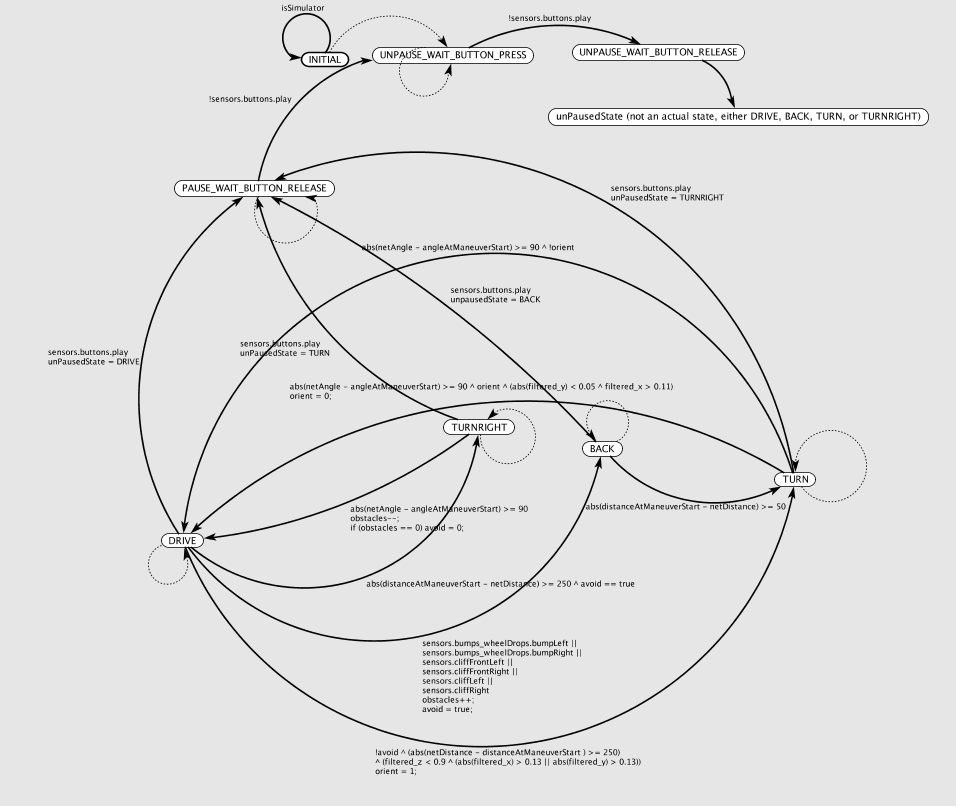
\includegraphics[width=\textwidth]{../lab5_data/FSMLab5}
    \end{center}
    
    % How did you account for movement of the robot when reading from the accelerometer? Describe any algorithms of filters used.
    To account for movement we would only take measurements for tilt after the robot was either in mid drive or mid turn. By doing this the robot should be close to constant velocity and have little effect on the tilt sensing.

    % Feedback
    We had two problems in this lab. One was that we assumed that the accelerometer data being fed to us was already filtered, since in the comments it said it was filtered. After we added our own filter the data was much more stable. Another problem we encountered was that the \texttt{abs()} function only takes integers as arguments. We were feeding in doubles, which did not produce the desired result. We made our own \texttt{absDouble()} function and this improved our algorithm dramatically.

  \section{Conclusion}
    This lab helped us further our use for state machines and also helped us think about how to use accelerometer data effectively. We learned how powerful state machines can be when used properly and how easy it is to change a state machine to add more functionality without having to rewrite the old code, we didn't change our obstacle avoidance state machine at all, only added to it. Learning to use the accelerometer data to sense tilt was very helpful, that way you don't need additional hardware to sense tilt.
\end{document}
